% Supplementary materials of article 1 (revised version v8). Build: latexmk -xelatex article1_v8_supplement.tex
\documentclass[12pt,a4paper]{article}
\usepackage[a4paper,top=2cm,bottom=2cm,left=3cm,right=1.5cm]{geometry}
\usepackage{fontspec}
\usepackage{polyglossia}
\setdefaultlanguage{russian}
\setotherlanguage{english}
\defaultfontfeatures{Ligatures=TeX}
\IfFontExistsTF{Times New Roman}{\setmainfont{Times New Roman}\newfontfamily\cyrillicfont{Times New Roman}}{\setmainfont{Liberation Serif}\newfontfamily\cyrillicfont{Liberation Serif}}
\usepackage{setspace}
\usepackage{mathtools,amssymb}
\usepackage{graphicx}
\usepackage{booktabs}
\usepackage{array}
\usepackage[unicode,hidelinks]{hyperref}
\setlength{\parindent}{1.25cm}
\onehalfspacing
\newcommand{\Psurr}{P_{\mathrm{surr}}}
\begin{document}

\begin{center}
{\large\bfseries Дополнительные материалы к статье}\\[4pt]
{\bfseries Сопряженность иерархических уровней атмосферной циркуляции как региональный инвариант}\\[4pt]
Н. С. Сотириади
\end{center}

\noindent Все расчеты воспроизводятся из открытого репозитория https://github.com/Theclimateguy/Shroedinger (релиз v6.5; маршрут -- reproducibility/article1\_README.md). Обозначения как в статье: $P$ -- исходный профиль, $\tilde P = P - \Psurr$ -- профиль с суррогатной поправкой; ступени 1--5 -- пары соседних полос от (мельче 50; 50--100 км) до (400--800; 800--1600 км).

\section*{П1. Полные профили двенадцати основных областей}

\noindent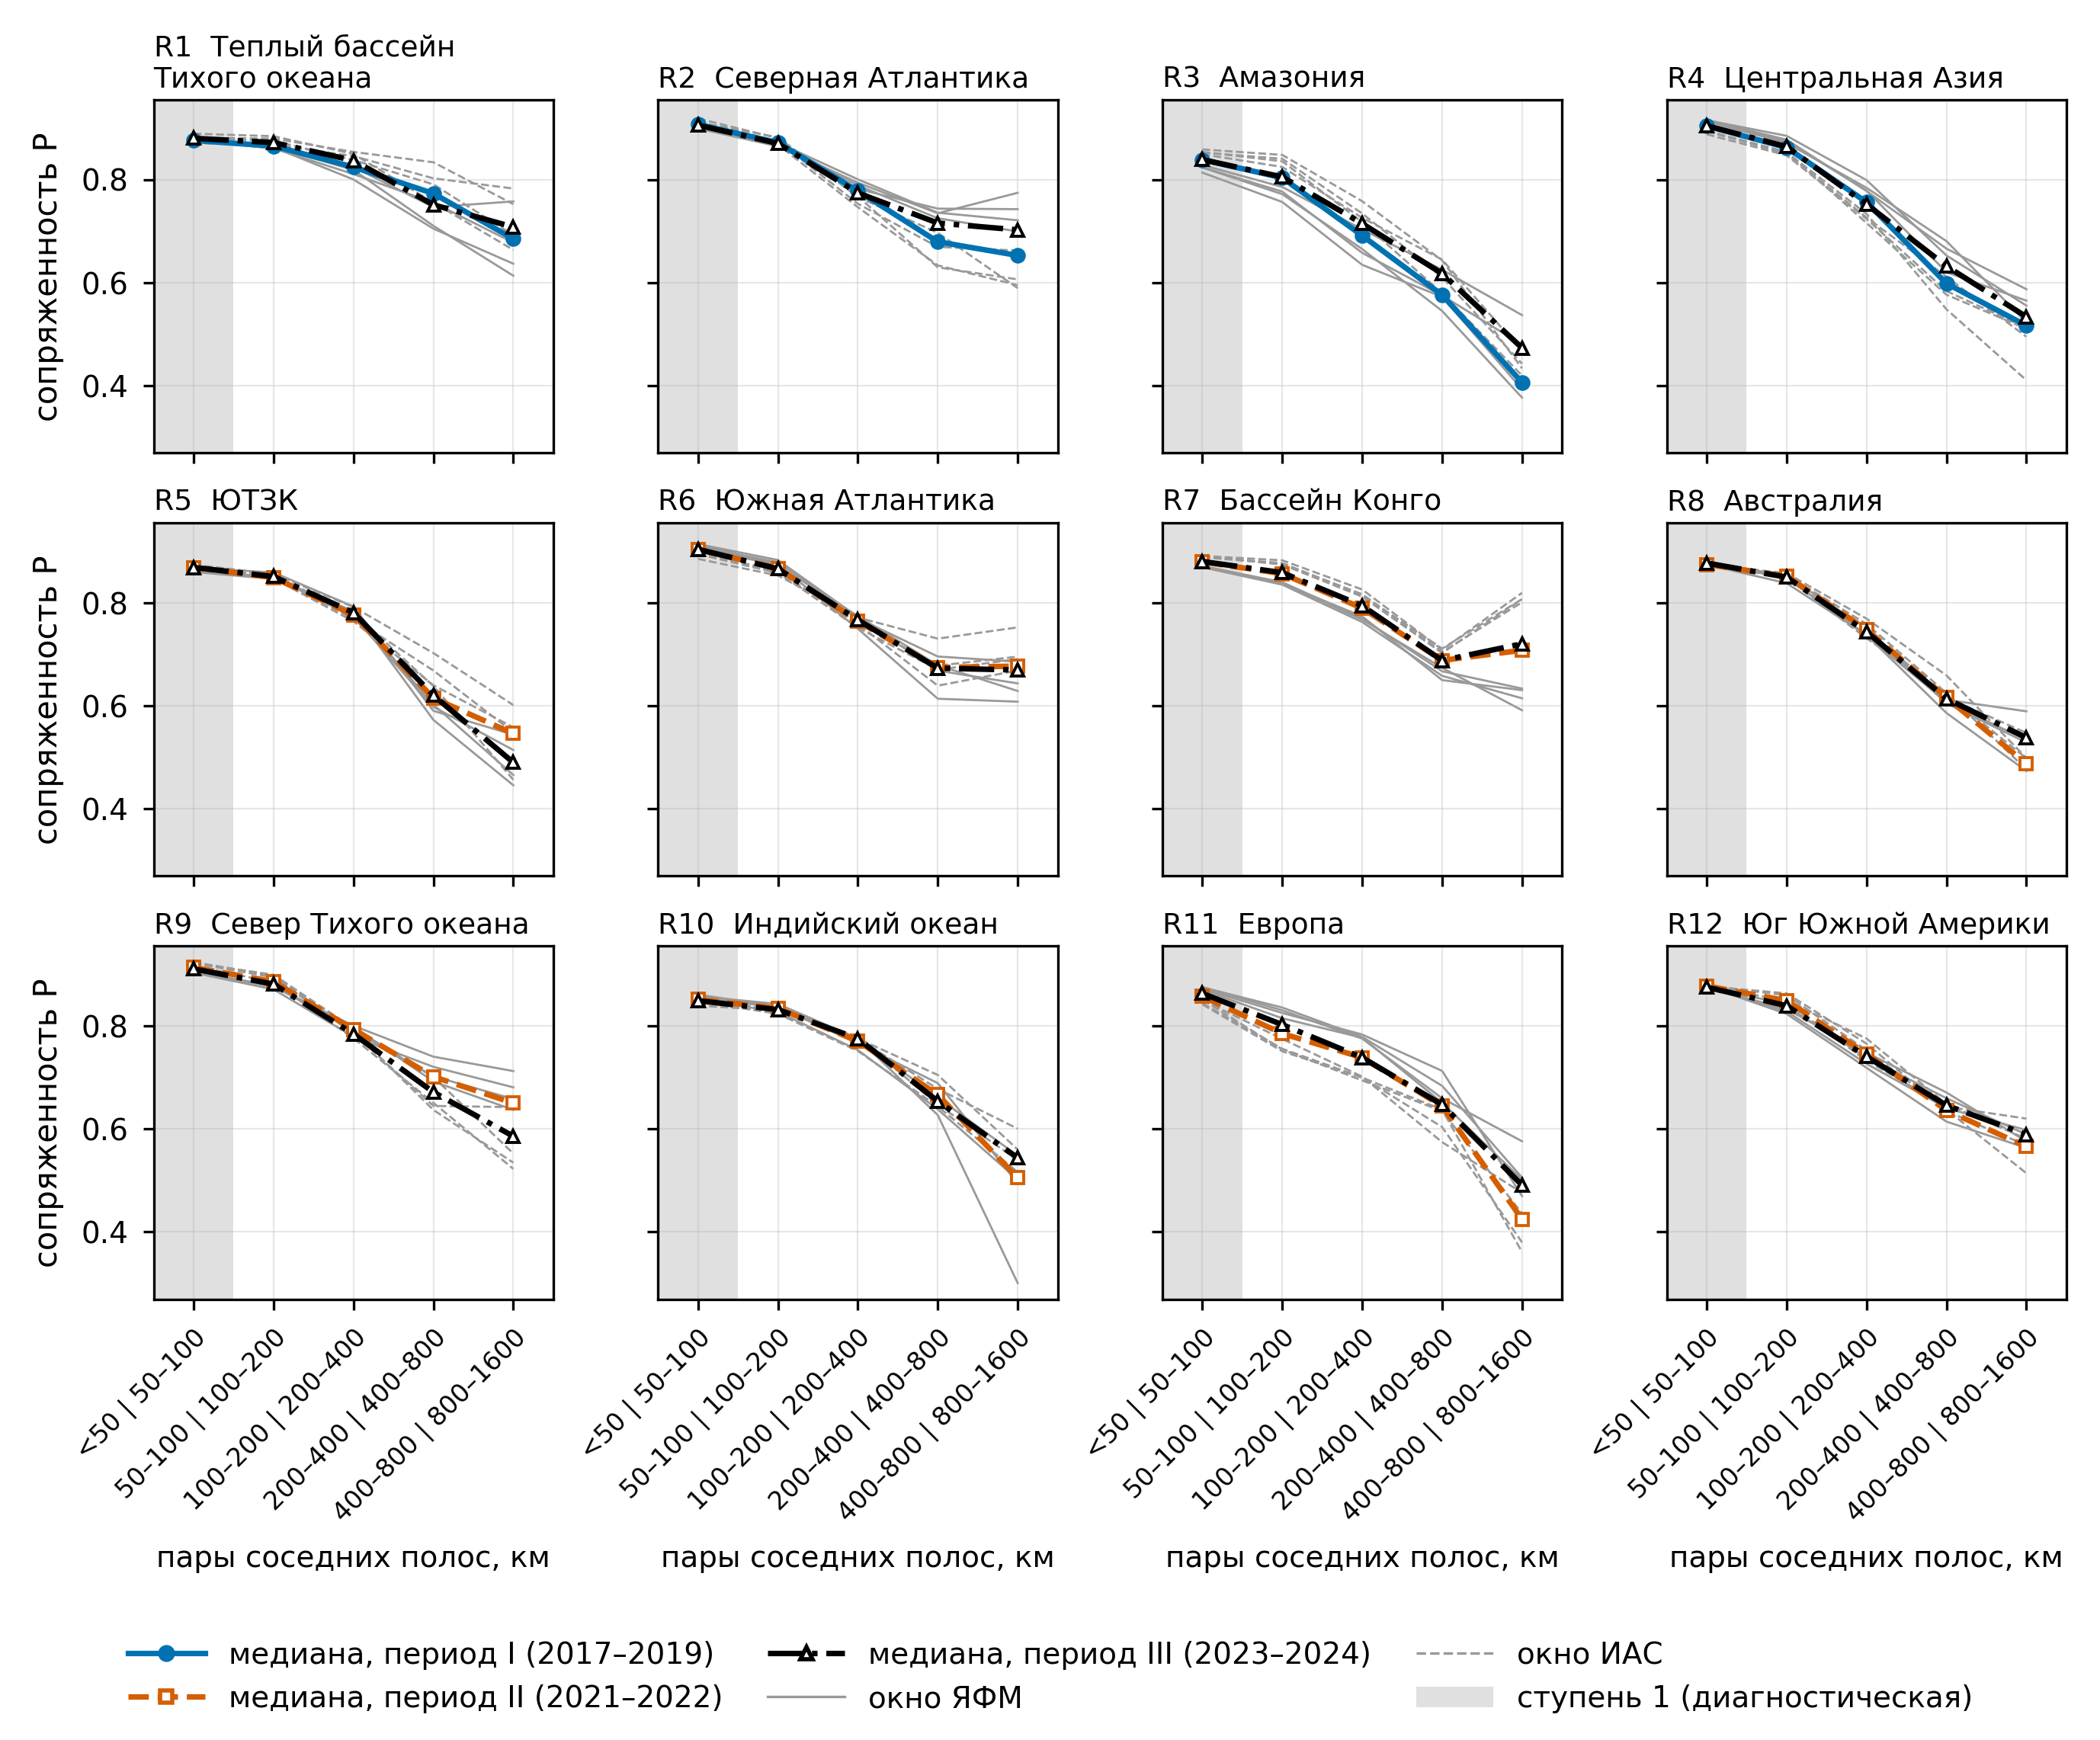
\includegraphics[width=\linewidth]{figures/v8/figA1_profiles_full_v8.png}

\noindent Рис. П1. Исходные профили $P$ по ступеням 1--5 для двенадцати основных областей (коды -- табл. 1 статьи): тонкие линии -- отдельные сезонные окна (сплошные -- январь--март, штриховые -- июль--сентябрь), жирные -- медианы по периодам 2017--2019, 2021--2022 и 2023--2024 гг. Серая полоса -- ступень 1 (пара полос мельче 100 км), исключенная из содержательных выводов: ее значение несет отпечаток анизотропии градусной сетки (связь с широтой 0.87 на градусной сетке против 0.65 на сетке с равным шагом в километрах; ступени 2--5 воспроизводятся на двух сетках с согласием 0.97--0.99).

\section*{П2. Контроль геометрии: градусные и равновеликие области}

\noindent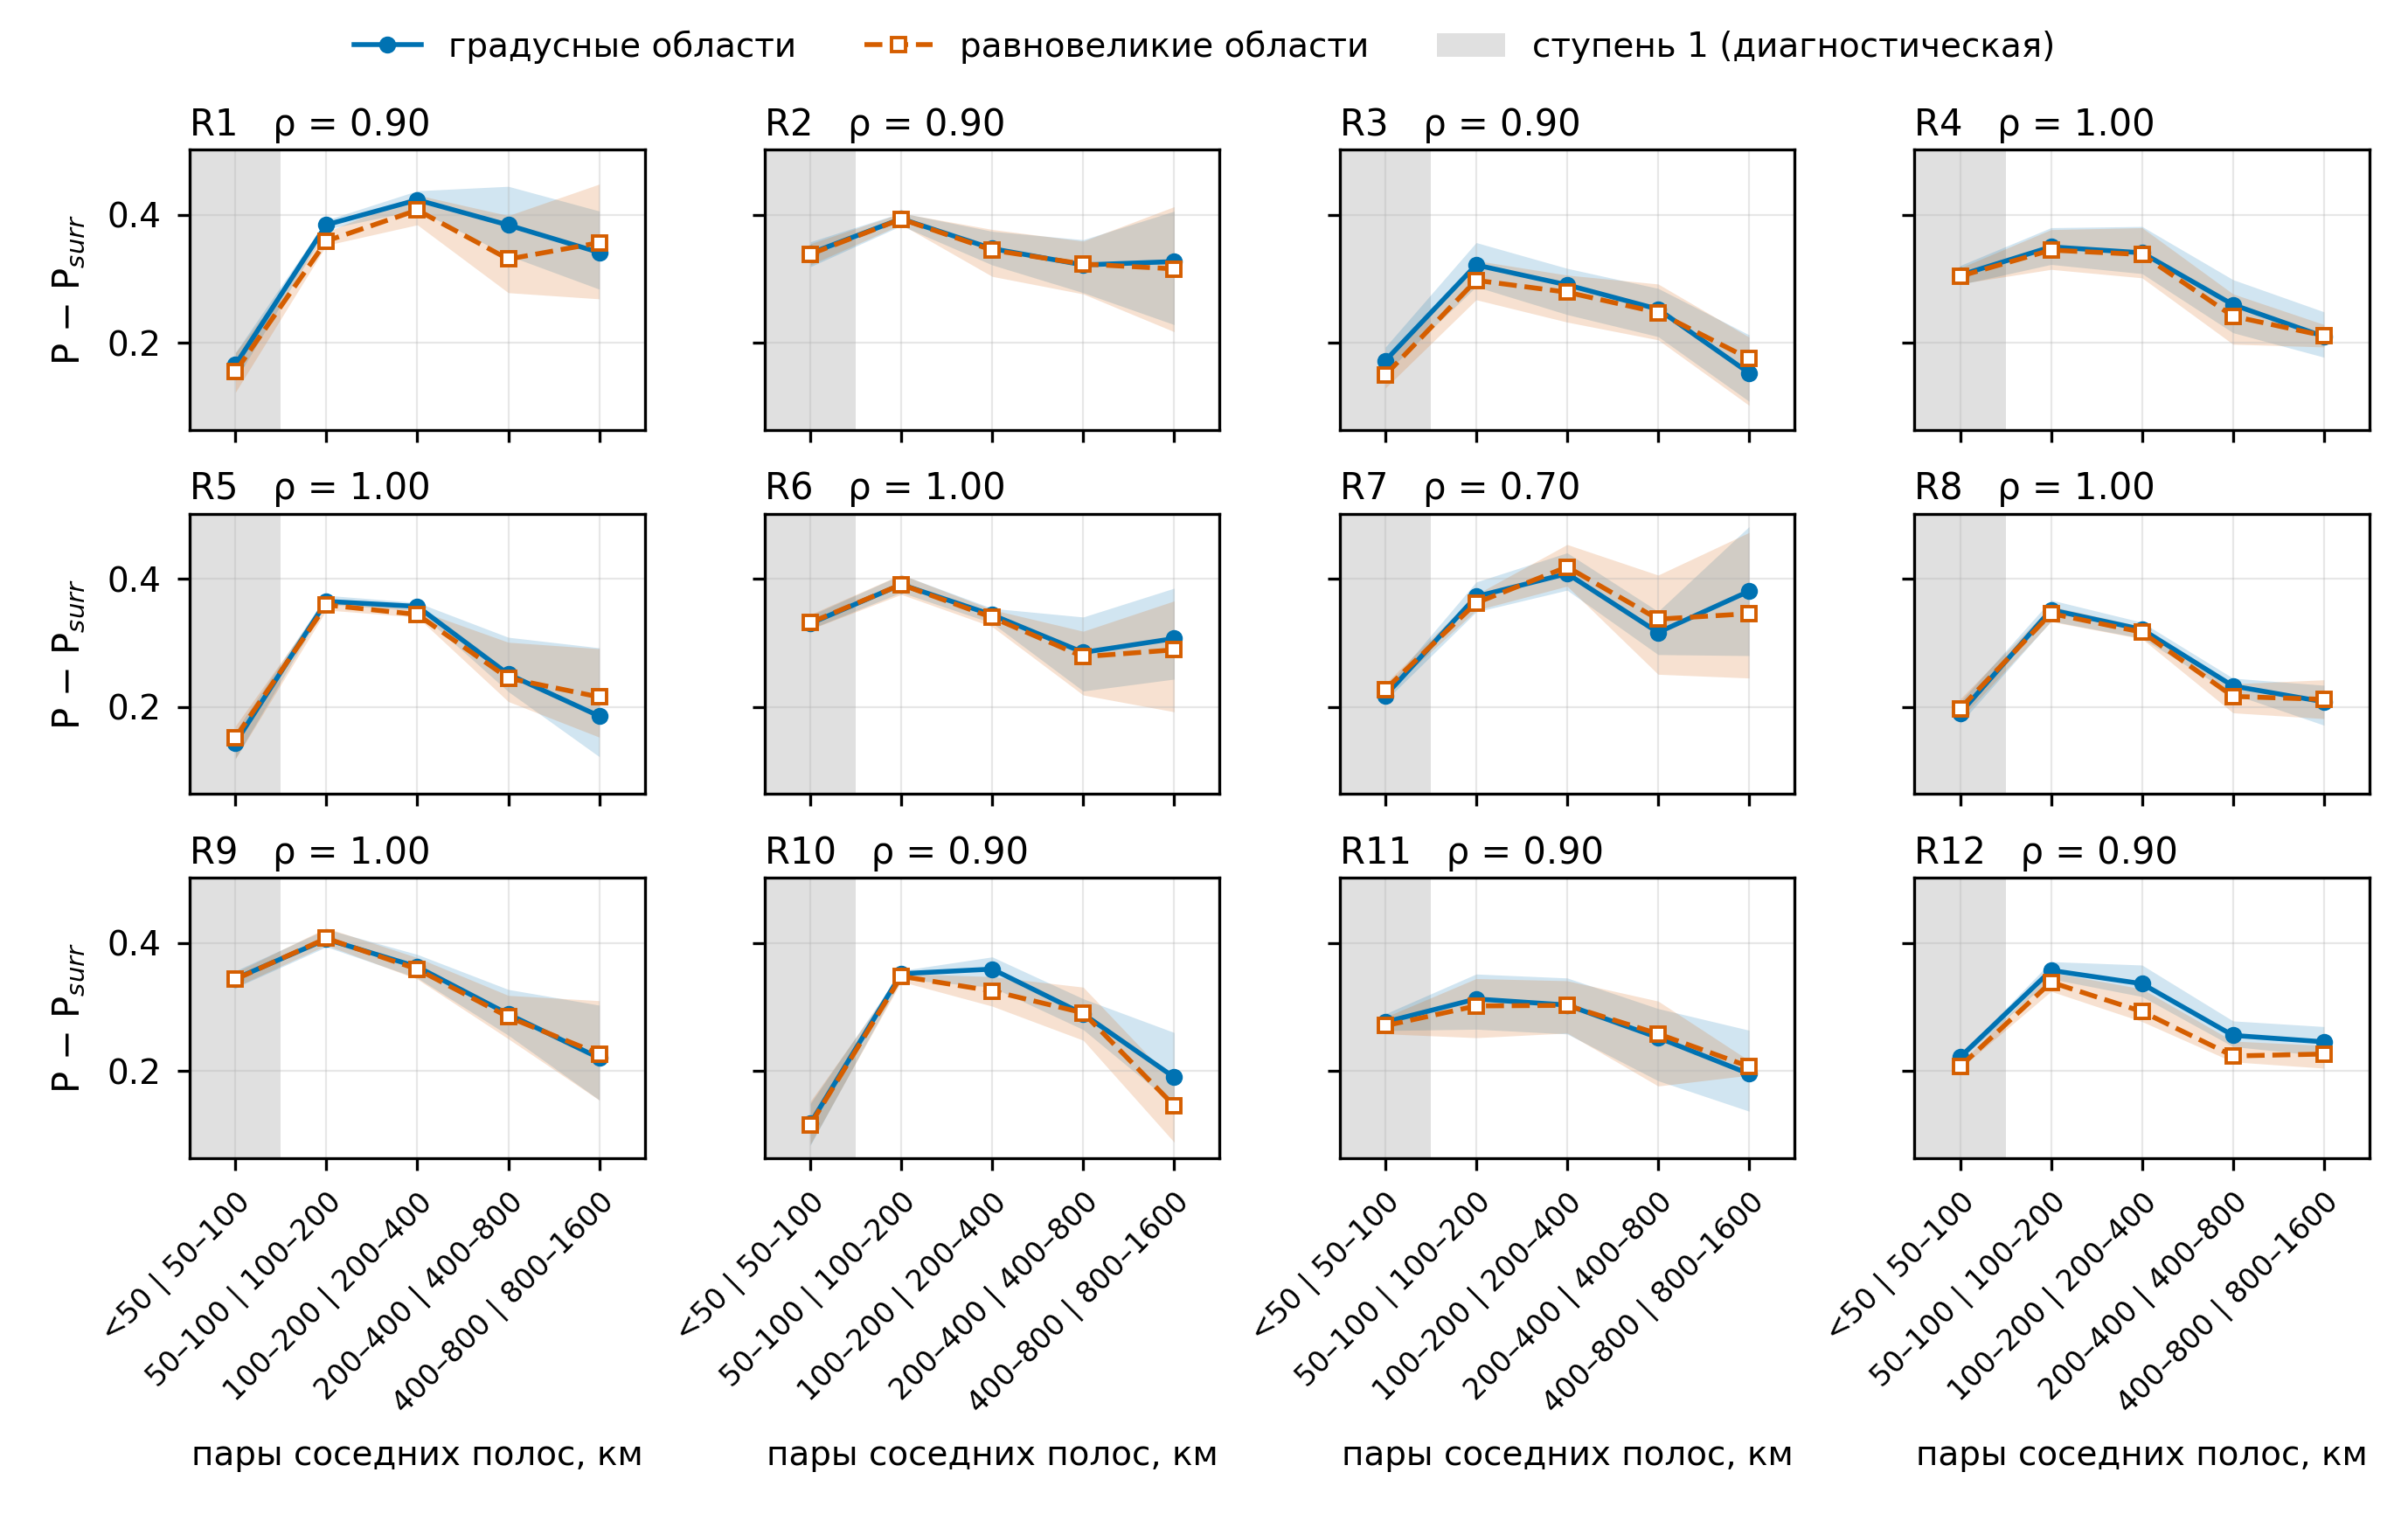
\includegraphics[width=\linewidth]{figures/v8/figA2_geometry_v8.png}

\noindent Рис. П2. Профили с суррогатной поправкой $\tilde P$ на градусных областях $20^\circ \times 40^\circ$ и на равновеликих областях $2000 \times 2800$ км (те же центры) для двенадцати регионов, 48 основных регион-окон 2023--2024 гг.: линии -- средние по окнам, полосы -- размах; в заголовках панелей -- ранговая корреляция профилей двух нарезок по региону (объединенная 0.95). Серая полоса -- ступень 1. Два дополнения той же серии проверок: лестница масштабов, умноженная на локальный радиус деформации (множители 0.65--2.0 по регионам), сохраняет группировку профиля с поправкой ($\Delta = +1.53$, $p = 0.001$); вариация зональной протяженности равновеликих областей на $\pm10\%$ воспроизводит профили каждого региона с $\rho \geq 0.95$.

\section*{П3. Свободный модельный расчет: дополнительные величины}

\noindent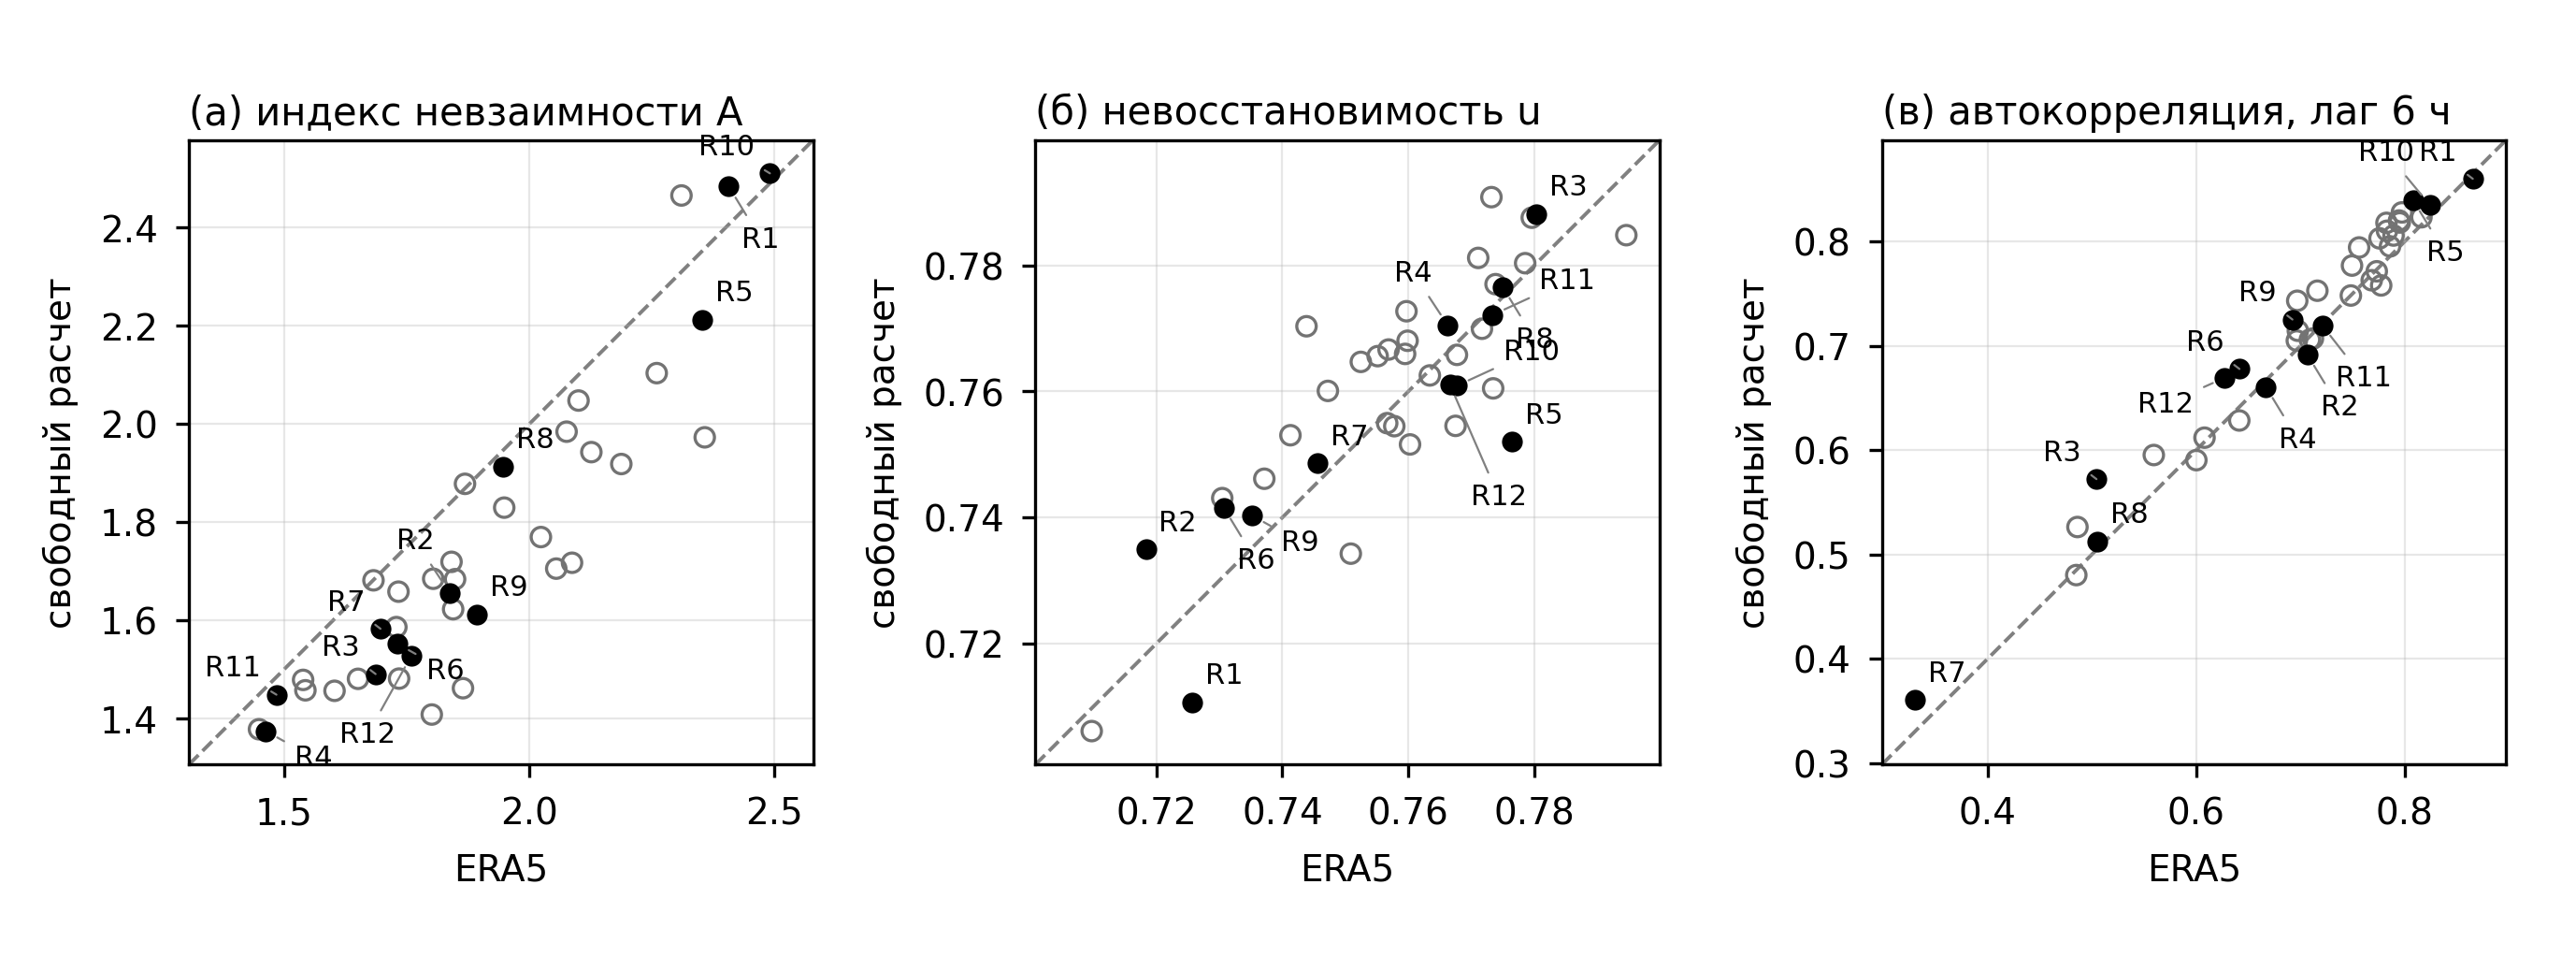
\includegraphics[width=\linewidth]{figures/v8/figA3_free_run_extra_v8.png}

\noindent Рис. П3. Сопоставление ERA5 и свободного расчета ECMWF-IFS-HR по 39 областям для величин, не вошедших в основной текст: индекс невзаимности $A$ (воспроизводим; его истолкование как меры необратимости обобщения отвергнуто), невосстановимость размещения $u$ (информационная мера раздела “Что измеряет величина”: ранги полей $E_{i-1}$ и $E_i$ по узлам внутренней части области разбиваются на $k = 16$ равночастотных корзин, по двумерной гистограмме вычисляется взаимная информация $I_i$, нормируемая на энтропию $H = \ln k$, $u_i = 1 - I_i/H$; медиана по срокам окна и среднее по разрешенным ступеням; связь с профилем $\rho = -0.86$; связь профиля с логарифмом дисперсии разрешенных полос $\rho = +0.13$ по 12 областям) и временная устойчивость карт активности (автокорреляция огибающей на лаге 6 ч). Ранговые корреляции: $A$ -- 0.90, $u$ -- 0.77, устойчивость -- 0.98.

\section*{П4. Полный перечень проверенных и отвергнутых интерпретаций}

\begin{singlespace}
\noindent\begin{tabular}{@{}p{0.5\linewidth}p{0.46\linewidth}@{}}
\toprule
Проверяемое положение & Итог проверки\\
\midrule
Индекс невзаимности $A$ измеряет необратимость географического обобщения & Отвергнуто (на синтетических полях индекс не реагирует на восстановимость мелкого уровня по крупному и следует за временной устойчивостью поля)\\
Профиль отслеживает межмасштабный поток кинетической энергии (метод пространственного огрубления) & Отвергнуто (объясняет доли процента изменчивости потока; характеристики поля деформации информативнее на два порядка)\\
Форма профилей подчиняется универсальному закону от средовых ковариат & Отвергнуто (коллапса к единой кривой нет)\\
Профиль вертикально универсален (перенос на 500 гПа) & Не подтверждено (при вдвое меньшей выборке)\\
Профиль информативен для замыкания влагобюджета реанализа & Отвергнуто\\
Режимная связь с осадками формализуема как уравнение “источник--сток” & Не установлено (характерное время $\sim$2 сут частично воспроизводится инерцией процедуры)\\
Профиль предсказывает скорость роста ошибки ансамблевого прогноза & Не подтверждено; сильнее предиктор -- бароклинность ($\rho = +0.86$ с модулем широты)\\
Профиль предсказывает уровень мезомасштабной ошибки анализа & Не подтверждено; связь исчезает после контроля амплитуды\\
Профиль предсказывает потерю мезомасштаба в нейросетевых моделях погоды & Не подтверждено; сильнее предиктор -- спектральная характеристика\\
Профиль содержит воспроизводимую информацию сверх спектра мощности (регрессионные остатки) & Неустойчиво (ступени 2--5): на 32 отложенных окнах $\Delta = +0.33$, $p = 0.011$; на всех 96 окнах $+0.40$, $p = 0.001$; на 48 основных окнах 2023--2024 гг. $\Delta \approx 0$, $p = 0.56$; тест на уровне областей для отложенных окон $p = 0.61$ -- открытый вопрос\\
\bottomrule
\end{tabular}
\end{singlespace}

\section*{П5. Чувствительность к определению поля: сферический ротор и маска 850 гПа}

\noindent Таблица П1. Доля узлов внутренней части области, в которых поверхность 850 гПа лежит под рельефом (ERA5: высота поверхности более 1457 м; MERRA-2: заполнители ниже поверхности).

\begin{singlespace}
\noindent\begin{tabular}{@{}lrr@{}}
\toprule
Область & ERA5, \% & MERRA-2, \%\\
\midrule
R4 Центральная Азия & 29 & 34\\
R7 Бассейн Конго & 7 & 3\\
R11 Европа & 5 & 1\\
R12 Юг Южной Америки & $<1$ (Анды в краевой полосе) & 7\\
R3 Амазония & $<1$ (Анды в краевой полосе) & 2\\
R1, R2, R5, R6, R8, R9, R10 & $<1$ & $<1$\\
\bottomrule
\end{tabular}
\end{singlespace}

\medskip
\noindent Таблица П2. Числа статьи до и после перехода к сферическому ротору и маске (все прочие параметры неизменны). Старое определение: локально-декартов ротор без маски; в MERRA-2 узлы под поверхностью заполнялись нулями.

\begin{singlespace}
\noindent\begin{tabular}{@{}p{0.5\linewidth}p{0.22\linewidth}p{0.22\linewidth}@{}}
\toprule
Величина & Старое определение & Сферический ротор + маска\\
\midrule
Сферическое слагаемое: изменение профиля, 48 окон 2023--2024 гг. & -- & $\le 0.009$ на любой ступени\\
Группировка на отложенных окнах, $P$, ступени 2--5 (1--5) & $+0.74$ ($+1.12$) & $+0.81$ ($+1.18$)\\
Только ступени 4--5, отложенные окна & $+0.50$, $p = 0.004$ & $+0.52$, $p = 0.002$\\
Равновеликие области, $\tilde P$, ступени 2--5: основные / отложенные & $+0.79$ / $+1.06$ & $+0.75$ / $+1.03$\\
MERRA-2: группировка / география с ERA5 & $+1.15$ / $0.86$ & $+1.09$ / $0.77$\\
Свободный расчет: география с ERA5 (39 областей) & $0.71$ & $0.72$\\
Ориентир ERA5 между периодами (8 / 12 областей) & $0.93$ / $0.92$ & $0.90$ / $0.95$\\
Конго / Амазония, ступень 5, медианы & $0.70$ / $0.42$ & $0.72$ / $0.44$\\
Центральная Азия, среднее ступеней 4--5 & $0.55$ & $0.57$\\
Ранговая корреляция старой и новой географии (12 областей, медианы по 8 окнам) & \multicolumn{2}{l}{$0.98$ (по окнам 2023--2024 гг.: $0.95$)}\\
\bottomrule
\end{tabular}
\end{singlespace}

\section*{П6. Компоненты дисперсии профиля}

\noindent Таблица П3. Разложение дисперсии исходного профиля $P$ по ступеням на 96 регион-окнах (12 областей $\times$ 8 окон): доля суммы квадратов, приходящаяся на регион, на сезон внутри региона и на год внутри региона и сезона (одно окно на ячейку, поэтому последний член совпадает с остатком); ICC -- коэффициент внутриклассовой корреляции одноуровневой модели.

\begin{singlespace}
\noindent\begin{tabular}{@{}lrrrr@{}}
\toprule
Ступень & Регион & Сезон & Год / остаток & ICC\\
\midrule
1 (диагностическая) & 0.86 & 0.12 & 0.02 & 0.85\\
2 & 0.70 & 0.27 & 0.03 & 0.68\\
3 & 0.65 & 0.28 & 0.07 & 0.63\\
4 & 0.61 & 0.23 & 0.16 & 0.58\\
5 & 0.69 & 0.17 & 0.14 & 0.67\\
\bottomrule
\end{tabular}
\end{singlespace}

\end{document}
